\documentclass[crop, tikz]{standalone}

\usepackage{tikz}
\usepackage{amsmath}
\usepackage{amssymb}
\usepackage[mode=buildnew]{standalone}

\usepackage{xcolor}


\usetikzlibrary{positioning}
\usetikzlibrary{calc}
\usetikzlibrary{fit}
%\usepackage{nicematrix}

\tikzset{set/.style={draw,circle,inner sep=0pt,align=center}}

\definecolor{morange}{RGB}{255,127,14}
\definecolor{mblue}{RGB}{31,119,180}
\definecolor{mred}{RGB}{214,39,40}
\definecolor{mpurple}{RGB}{148,103,189}
\definecolor{mgreen}{RGB}{44,160,44}


\begin{document}
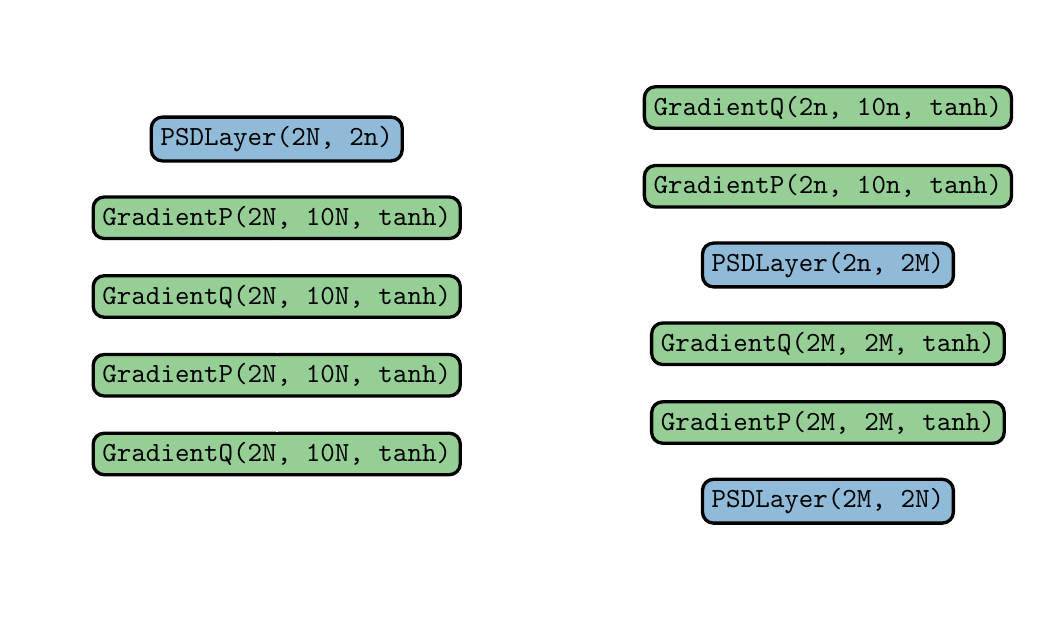
\begin{tikzpicture}[module/.style={draw, very thick, rounded corners, minimum width=15ex},
    gradient/.style={module, fill=mgreen!50},
    psd/.style={module, fill=mblue!50},
    arrow/.style={-stealth, thick, rounded corners},
]
\node (input) {\color{white} Input};
\node[above of=input, gradient, align=center, yshift=.6cm] (gq1) {\texttt{GradientQ(2N, 10N, tanh)}};
\node[above of=gq1, gradient, align=center] (gq2) {\texttt{GradientP(2N, 10N, tanh)}};
\node[above of=gq2, gradient, align=center] (gq3) {\texttt{GradientQ(2N, 10N, tanh)}};
\node[above of=gq3, gradient, align=center] (gq4) {\texttt{GradientP(2N, 10N, tanh)}};
\node[above of=gq4, psd, align=center] (psd1) {\texttt{PSDLayer(2N, 2n)}};

\node[right of=input, xshift=6cm] (output) {\color{white} Output}; 
\node[above of=output, psd] (psd3) {\texttt{PSDLayer(2M, 2N)}};
\node[above of=psd3, gradient] (gq8) {\texttt{GradientP(2M, 2M, tanh)}};
\node[above of=gq8, gradient] (gq7) {\texttt{GradientQ(2M, 2M, tanh)}};
\node[above of=gq7, psd] (psd2) {\texttt{PSDLayer(2n, 2M)}};
\node[above of=psd2, gradient] (gq6) {\texttt{GradientP(2n, 10n, tanh)}};
\node[above of=gq6, gradient] (gq5) {\texttt{GradientQ(2n, 10n, tanh)}};

\draw[arrow, color=white] (gq1) -- (gq2);
\draw[arrow, color=white] (gq2) -- (gq3); 
\draw[arrow, color=white] (gq3) -- (gq4);
\draw[arrow, color=white] (gq4) -- (psd1); 

\coordinate[above of=gq5] (gq5_above);
\coordinate[left of=gq5_above, xshift=-6cm] (psd_above);

\draw[arrow, color=white] (gq5) -- (gq6);
\draw[arrow, color=white] (gq6) -- (psd2);
\draw[arrow, color=white] (psd2) -- (gq7);
\draw[arrow, color=white] (gq7) -- (gq8);
\draw[arrow, color=white] (gq8) -- (psd3);

\node[fit=(gq1)(gq2)(gq3)(gq4)(psd1),draw, ultra thick, rounded corners, color=white, label=left:\color{white}$\Psi^e$] (encoder) {};
\node[fit=(gq5)(gq5)(gq7)(psd2)(gq7)(gq8)(psd3),draw, ultra thick, rounded corners, color=white, label=left:\color{white}$\Psi^d$] (decoder) {};

\draw[arrow, color=white] (encoder.north)-|(psd_above)-|(gq5_above)--(decoder.north);
\draw[arrow, color=white] (input) -- (encoder);
\draw[arrow, color=white] (decoder) -- (output);


\end{tikzpicture}
\end{document}